\chapter{Immutable Objects}
\label{immutable}

\index{object-oriented}

Java is an ``object-oriented'' language, which means that it uses objects to (1)~represent data and (2)~provide methods related to them.
This way of organizing programs is a powerful design concept, and we will introduce it gradually throughout the remainder of the book.

\index{object}
\index{System.in}
\index{System.out}

An {\bf object} is a collection of data that provides a set of methods.
For example, \java{Scanner}, which we saw in Section~\ref{scanner}, is an object that provides methods for parsing input.
\java{System.out} and \java{System.in} are also objects.

Strings are objects, too.
They contain characters and provide methods for manipulating character data.
Other data types, like \java{Integer}, contain numbers and provide methods for manipulating number data.
We will explore some of these methods in this chapter.


\section{Primitives vs Objects}

\index{primitive}

Not everything in Java is an object: \java{int}, \java{double}, \java{char}, and \java{boolean} are {\bf primitive} types.
%We will explain some of the differences between object types and primitive types as we go along.
When you declare a variable with a primitive type, Java reserves a small amount of memory to store its value.
Figure~\ref{fig.mem1} shows how the following values are stored in memory.

\begin{code}
int number = -2;
char symbol = '!';
\end{code}

\begin{figure}[!ht]
\begin{center}
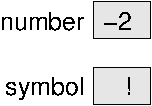
\includegraphics[width=80pt]{figs/mem1.pdf}
\caption{Memory diagram of two primitive variables.}
\label{fig.mem1}
\end{center}
\end{figure}

\index{memory diagram}
\index{diagram!memory}

As we learned in Section~\ref{elements}, an array variable stores a {\em reference} to an array.
%That's because the array itself is too large to fit in the variable's memory.
For example, the following line declares a variable named \java{array} and creates an array of three characters.

\begin{code}
    char[] array = {'c', 'a', 't'};
\end{code}

Figure~\ref{fig.mem2} shows them both, with a box to represent the location of the variable and an arrow pointing to the location of the array.

\begin{figure}[!ht]
\begin{center}
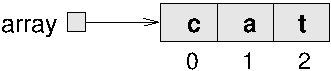
\includegraphics[width=205pt]{figs/mem2.pdf}
\caption{Memory diagram of an array of characters.}
\label{fig.mem2}
\end{center}
\end{figure}

Objects work in a similar way.
For example, this line declares a \java{String} variable named \java{word} and creates a \java{String} object, as shown in Figure~\ref{fig.mem3}.

\begin{code}
String word = "dog";
\end{code}

\begin{figure}[!ht]
\begin{center}
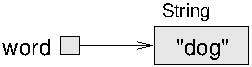
\includegraphics[width=160pt]{figs/mem3.pdf}
\caption{Memory diagram of a \java{String} object.}
\label{fig.mem3}
\end{center}
\end{figure}

Objects and arrays are usually created with the \java{new} keyword, which allocates memory for them. %(see Section~\ref{allocate})
For convenience, you don't have to use \java{new} to create strings:

\begin{code}
String word = new String("dog");  // creates a string object
String word = "dog";   // implicitly creates a string object
\end{code}

\index{string!comparing}

Recall from Section~\ref{strcmp} that you need to use the \java{equals} method to compare strings.
The \java{equals} method traverses the \java{String} objects and tests whether they contain the same characters.

To test whether two integers or other primitive types are equal, you can simply use the \java{==} operator.
But two \java{String} objects with the same characters would not be considered equal in the \java{==} sense.
The \java{==} operator, when applied to string variables, only tests whether they refer to the {\em same} object.


\section{The null Keyword}

Often when you declare an object variable, you assign it to reference an object.
But sometimes you want to declare variable that doesn't refer to an object, at least initially.

\index{null}

In Java, the keyword \java{null} is a special value that means ``no object''.
You can initialize object and array variables this way:

\begin{code}
String name = null;
int[] combo = null;
\end{code}

The value \java{null} is represented in memory diagrams by a small box with no arrow, as in Figure~\ref{fig.mem4}.

\begin{figure}[!ht]
\begin{center}
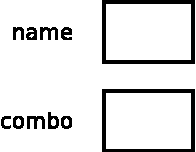
\includegraphics[width=80pt]{figs/mem4.pdf}
\caption{Memory diagram showing variables that are \java{null}.}
\label{fig.mem4}
\end{center}
\end{figure}

\index{NullPointerException}
\index{exception!NullPointer}

If you try to use a variable that is \java{null} by invoking a method or accessing an element, Java throws a \java{NullPointerException}.

\begin{code}
System.out.println(name.length());  // NullPointerException
System.out.println(combo[0]);       // NullPointerException
\end{code}

On the other hand, it is perfectly fine to pass a \java{null} reference as an argument to a method, or to receive one as a return value.
In these situations, \java{null} is often used to represent a special condition or indicate an error.


\section{Strings are Immutable}

If the Java library didn't have a \java{String} class, we would have to use character arrays to store and manipulate text.
Operations like concatenation~(\java{+}), \java{indexOf}, and \java{substring} would be difficult and inconvenient.
Fortunately, Java does have a \java{String} class that provides these and other methods.

\index{toUpperCase}
\index{toLowerCase}
\index{immutable}

For example, the methods \java{toLowerCase} and \java{toUpperCase} convert uppercase letters to lowercase, and vice versa.
These methods are often a source of confusion, because it sounds like they modify strings.
But neither these methods nor any others can change a string, because strings are {\bf immutable}.

When you invoke \java{toUpperCase} on a string, you get a new \java{String} object as a result.
For example:

\begin{code}
String name = "Alan Turing";
String upperName = name.toUpperCase();
\end{code}

%\index{Turing, Alan}

After these statements run, \java{upperName} refers to the string \java{"ALAN TURING"}.
But \java{name} still refers to \java{"Alan Turing"}.
A common mistake is to assume that \java{toUpperCase} somehow affects the original string:

\begin{code}
String name = "Alan Turing";
name.toUpperCase();           // ignores the return value
System.out.println(name);
\end{code}

The previous code displays \java{"Alan Turing"}, because the value of \java{name}, which refers to the original \java{String} object, never changes.
If you want to change \java{name} to be uppercase, then you need to assign the return value:

\begin{code}
String name = "Alan Turing";
name = name.toUpperCase();    // references the new string
System.out.println(name);
\end{code}

\index{replace}

A similar method is \java{replace}, which finds and replaces instances of one string within another.
This example replaces \java{"Computer Science"} with \java{"CS"}:

\begin{code}
String text = "Computer Science is fun!";
text = text.replace("Computer Science", "CS");
\end{code}

%This example demonstrates a common way to work with string methods.
%It invokes \java{text.replace}, which returns a reference to a new string, \java{"CS is fun!"}.
%Then it assigns the new string to \java{text}, replacing the old string.

As with \java{toUpperCase}, assigning the return value (to \java{text}) is important.
If you don't assign the return value, invoking \java{text.replace} has no effect.

Strings are immutable by design, because it simplifies passing them as parameters and return values.
And since the contents of a string can never change, two variables can reference the same string without one accidentally corrupting the other.


\section{Wrapper Classes}

Primitive types like \java{int}, \java{double}, and \java{char} cannot be \java{null}, and they do not provide methods.
For example, you can't invoke \java{equals} on an \java{int}:

\begin{code}
int i = 5;
System.out.println(i.equals(5));  // compiler error
\end{code}

\index{wrapper class}
\index{class!wrapper}
\index{Character}
\index{Integer}
\index{Double}

But for each primitive type, there is a corresponding {\bf wrapper class} in the Java library.
The wrapper class for \java{int} is named \java{Integer}, with a capital \java{I}.

\begin{code}
Integer i = new Integer(5);
System.out.println(i.equals(5));  // displays true
\end{code}

Other wrapper classes include \java{Boolean}, \java{Character}, \java{Double}, and \java{Long}.
They are in the \java{java.lang} package, so you can use them without importing them.

Like strings, objects from wrapper classes are immutable, and you have to use the \java{equals} method to compare them.

\begin{code}
Integer x = new Integer(123);
Integer y = new Integer(123);
if (x == y) {                     // false
    System.out.println("x and y are the same object");
}
if (x.equals(y)) {                // true
    System.out.println("x and y have the same value");
}
\end{code}

Because \java{x} and \java{y} refer to different objects, this code only displays ``x and y have the same value''.

Each wrapper class defines the constants \java{MIN_VALUE} and \java{MAX_VALUE}.
For example, \java{Integer.MIN_VALUE} is \java{-2147483648}, and \java{Integer.MAX_VALUE} is \java{2147483647}.
Because these constants are available in wrapper classes, you don't have to remember them, and you don't have to write them yourself.

\index{parse}

Wrapper classes also provide methods for converting strings to and from primitive types.
For example, \java{Integer.parseInt} converts a string to an \java{int}.
In this context, {\bf parse} means ``read and translate''.

\begin{code}
String str = "12345";
int num = Integer.parseInt(str);
\end{code}

Other wrapper classes provide similar methods, like \java{Double.parseDouble} and \java{Boolean.parseBoolean}.
They also provide \java{toString}, which returns a string representation of a value:

\begin{code}
int num = 12345;
String str = Integer.toString(num);
\end{code}

The result is the \java{String} object \java{"12345"}.

\index{NumberFormatException}
\index{exception!NumberFormat}

It's always possible to convert a primitive value to a string, but not the other way around.  For example, if we try to parse an invalid string like this:

\begin{code}
String str = "five";
int num = Integer.parseInt(str);  // NumberFormatException
\end{code}

\java{parseInt} throws a \java{NumberFormatException}, because the characters in the string \java{"five"} are not digits.


\section{Command-Line Arguments}

\index{args}
\index{command-line interface}

Now that you know about strings, arrays, and wrapper classes, we can {\em finally} explain the \java{args} parameter of the \java{main} method, which we have been ignoring since Chapter~\ref{theway}.
If you are unfamiliar with the command-line interface, please read Appendix~\ref{commandline}.

Let's write a program to find the maximum value in a sequence of numbers.
Rather than read the numbers from \java{System.in} using a \java{Scanner}, we'll pass them as command-line arguments.
Here is a starting point:

\begin{code}
import java.util.Arrays;
public class Max {
    public static void main(String[] args) {
        System.out.println(Arrays.toString(args));
    }
}
\end{code}

You can run this program from the command line by typing:

\begin{stdout}
java Max
\end{stdout}

\index{empty array}

The output indicates that \java{args} is an {\bf empty array}; that is, it has no elements:

\begin{stdout}
[]
\end{stdout}

If you provide additional values on the command line, they are passed as arguments to \java{main}.
For example, if you run the program like this:

\begin{stdout}
java Max 10 -3 55 0 14
\end{stdout}

The output is:

\begin{stdout}
[10, -3, 55, 0, 14]
\end{stdout}

It's not clear from the output, but the elements of \java{args} are strings.
So \java{args} is the array \java{\{"10", "-3", "55", "0", "14"\}}.
To find the maximum number, we have to convert the arguments to integers.

The following code uses an enhanced \java{for} loop (see Section~\ref{enhanced}) to parse the arguments and find the largest value:

\begin{code}
int max = Integer.MIN_VALUE;
for (String arg : args) {
    int value = Integer.parseInt(arg);
    if (value > max) {
        max = value;
    }
}
System.out.println("The max is " + max);
\end{code}

We begin by initializing \java{max} to the smallest (most negative) number an \java{int} can represent.
That way, the first value we parse will replace \java{max}.
As we find larger values, they will replace \java{max} as well.

If \java{args} is empty, the result will be \java{MIN_VALUE}.
We can prevent this situation from happening by checking \java{args} at the beginning of the program:

\begin{code}
if (args.length == 0) {
    System.err.println("Usage: java Max <numbers>");
    return;
}
\end{code}

It's customary for programs that require command-line arguments to display a ``usage'' message if the arguments are not valid.
For example, if you run {\tt javac} or {\tt java} from the command line without any arguments, you will get a very long message.


\section{Argument Validation}

As we discussed in Section~\ref{validate}, you should never assume that program input will be in the correct format.
Sometimes users make mistakes, such as pressing the wrong key or misreading instructions.

\index{hacker}

Or even worse, someone might make intentional ``mistakes'' to see what your program will do.
One way hackers break into computer systems is by entering malicious input that causes a program to fail.

Programmers can make mistakes too.
It's difficult to write bug-free software, especially when working in teams on large projects.

\index{validate}

For all of these reasons, it's good practice to validate arguments passed to methods, including the \java{main} method.
In the previous section, we did this by ensuring that \java{args.length} was not zero.

\index{Character}

As a further example, consider a method that checks whether the first word of a sentence is capitalized.
We can write this method using the \java{Character} wrapper class:

\begin{code}
public static boolean isCapitalized(String str) {
    return Character.isUpperCase(str.charAt(0));
}
\end{code}

The expression \java{str.charAt(0)} makes two assumptions: the string object referenced by \java{str} exists, and it has at least one character.
What if these assumptions don't hold at run-time?

\begin{itemize}

\index{NullPointerException}
\index{exception!NullPointer}

\item If \java{str} is \java{null}, invoking \java{charAt} will cause a \java{NullPointerException}, because you can't invoke a method on \java{null}.

\index{StringIndexOutOfBoundsException}
\index{exception!StringIndexOutOfBounds}

\item If \java{str} refers to an empty string, which is a \java{String} object with no characters, \java{charAt} will cause a \java{StringIndexOutOfBoundsException}, because there is no character at index \java{0}.

\end{itemize}

We can prevent these exceptions by validating \java{str} {\em at the start} of the method.
If it's invalid, we return before executing the rest of the method.

\begin{code}
public static boolean isCapitalized(String str) {
    if (str == null || str.isEmpty()) {
        return false;
    }
    return Character.isUpperCase(str.charAt(0));
}
\end{code}

Notice that \java{null} and ``empty'' are different concepts, as shown in Figure~\ref{fig.nullempty}.
The variable \java{str1} is \java{null}, meaning that it doesn't reference an object.
The variable \java{str2} refers to the empty string, an object that exists.
%Internally, the empty string is stored as a \java{char} array of length zero (represented by a small box).

\begin{figure}[!ht]
\begin{center}
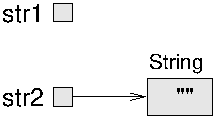
\includegraphics[width=155pt]{figs/nullempty.pdf}
\caption{Memory diagram of \java{null} and empty string.}
\label{fig.nullempty}
\end{center}
\end{figure}

Beginners sometimes make the mistake of checking for empty first.
Doing so causes a \java{NullPointerException}, because you can't invoke methods on variables that are \java{null}.

\begin{code}
if (str.isEmpty() || str == null) {    // wrong!
\end{code}

\index{short circuit}

Checking for \java{null} first prevents the \java{NullPointerException}.
If \java{str} is \java{null}, the \java{||} operator will short circuit (see Section~\ref{shortcircuit}) and evaluate to \java{true} immediately.
As a result, \java{str.isEmpty()} will not be called.


\section{BigInteger Arithmetic}
% CSM based on text from V6 Exercise 10.4

It might not be clear at this point why you would ever need an integer object when you can just use an \java{int} or \java{long}.
One advantage is the variety of methods that \java{Integer} and \java{Long} provide.
But there is another reason: when you need very large integers that exceed \java{Long.MAX_VALUE}.

\index{BigInteger}

\java{BigInteger} is a Java class that can represent arbitrarily large integers.
There is no upper bound except the limitations of memory size and processing speed.
Take a minute to read the documentation, which you can find by doing a web search for ``Java BigInteger''.

% ABD: Now that we have short links, should we add one here rather than
% tell people how to look for it?

\index{java.math}

To use BigIntegers, you have to \java{import java.math.BigInteger} at the beginning of your program.
There are several ways to create a BigInteger, but the simplest uses \java{valueOf}.
The following code converts a \java{long} to a BigInteger:

\begin{code}
long x = 17;
BigInteger big = BigInteger.valueOf(x);
\end{code}

You can also create BigIntegers from strings.
For example, here is a 20-digit integer that is too big to store using a \java{long}.

\begin{code}
String s = "12345678901234567890";
BigInteger bigger = new BigInteger(s);
\end{code}

Notice the difference in the previous two examples: you use \java{valueOf} to convert integers, and \java{new BigInteger} to convert strings.

Since BigIntegers are not primitive types, the usual math operators don't work.
Instead, we have to use methods like \java{add}.
To add two BigIntegers, we invoke \java{add} on one and pass the other as an argument.

\begin{code}
BigInteger a = BigInteger.valueOf(17);
BigInteger b = BigInteger.valueOf(1700000000);
BigInteger c = a.add(b);
\end{code}

Like strings, \java{BigInteger} objects are immutable.
Methods like \java{add}, \java{multiply}, and \java{pow} all return new BigIntegers, rather than modify an existing one.

Internally, a BigInteger is implemented using an array of \java{int}s, similar to the way a string is implemented using an array of \java{char}s.
Each \java{int} in the array stores a portion of the BigInteger.
The methods of \java{BigInteger} traverse this array to perform addition, multiplication, etc.

For very long floating-point values, take a look at \java{java.math.BigDecimal}.
Interestingly, \java{BigDecimal} objects represent floating-point numbers internally using a \java{BigInteger}!

% ABD: I think explaining the implementation here is a good idea.
% The level of detail is appropriate, and it explains what might
% otherwise seem like magic.


\section{Incremental Design}
\label{encapsulation}

%This chapter introduces two main concepts: objects encapsulate other types of data, and they can be designed to be immutable.
%Applying these concepts helps us to manage the complexity of programs as they become large.

%Unfortunately, computer science has a lot of overloaded terms.
%Another use of the term ``encapsulation'' applies to methods.

\index{design process}
\index{encapsulation!and generalization}

One challenge of programming, especially for beginners, is figuring out how to divide a program into methods.
In this section, we present a {\bf design process} that allows you to divide a program into methods as you go along.
The process is called ``encapsulation and generalization''.
The essential steps are:

\begin{enumerate}
\item Write a few lines of code in \java{main} or another method, and test them.
\item When they are working, wrap them in a new method, and test again.
\item If it's appropriate, replace literal values with variables and parameters.
\end{enumerate}

\index{table!two-dimensional}

To demonstrate this process, we'll develop methods that display multiplication tables.
We begin by writing and testing a few lines of code.
Here is a loop that displays the multiples of two, all on one line:

\begin{code}
for (int i = 1; i <= 6; i++) {
    System.out.printf("%4d", 2 * i);
}
System.out.println();
\end{code}

%\index{loop variable}
%\index{variable!loop}
%
%The first line initializes a variable named \java{i}, which is going to act as the loop variable.
%As the loop executes, the value of \java{i} increases from 1 to 6; when \java{i} is 7, the loop terminates.

Each time through the loop, we display the value of \java{2 * i}, padded with spaces so it's four characters wide.
Since we use \java{System.out.printf}, the output appears on a single line.

After the loop, we call \java{println} to print a newline character.
Remember that in some environments, none of the output is displayed until the line is complete.
The output of the code so far is:

\begin{stdout}
   2   4   6   8  10  12
\end{stdout}

\index{encapsulate}

The next step is {\bf encapsulation}; that is, we ``wrap'' the code in a method:

\begin{code}
public static void printRow() {
    for (int i = 1; i <= 6; i++) {
        System.out.printf("%4d", 2 * i);
    }
    System.out.println();
}
\end{code}

\index{generalize}

Finally, we generalize the method to print multiples of other numbers by replacing the constant value \java{2} with a parameter \java{n}.
This step is called {\bf generalization}, because it makes the method more general (less specific).

\begin{code}
public static void printRow(int n) {
    for (int i = 1; i <= 6; i++) {
        System.out.printf("%4d", n * i);  // generalized n
    }
    System.out.println();
}
\end{code}

Invoking this method with the argument \java{2} yields the same output as before.
With the argument \java{3}, the output is:

\begin{stdout}
   3   6   9  12  15  18
\end{stdout}

%And with argument 4, the output is:
%
%\begin{stdout}
%   4   8  12  16  20  24
%\end{stdout}

By now you can probably guess how we are going to display a multiplication table: we'll invoke \java{printRow} repeatedly with different arguments.
In fact, we'll use another loop to iterate through the rows.

\begin{code}
for (int i = 1; i <= 6; i++) {
    printRow(i);
}
\end{code}

And the output looks like this:

\begin{stdout}
   1   2   3   4   5   6
   2   4   6   8  10  12
   3   6   9  12  15  18
   4   8  12  16  20  24
   5  10  15  20  25  30
   6  12  18  24  30  36
\end{stdout}

%The format specifier \java{\%4d} in \java{printRow} causes the output to align vertically, regardless of whether the numbers are one or two digits.


\section{More Generalization}

The previous result is similar to the ``nested loops'' approach in Section~\ref{nested}.
However, the inner loop is now encapsulated in the \java{printRow} method.
We can encapsulate the outer loop in a method too:

\begin{code}
public static void printTable() {
    for (int i = 1; i <= 6; i++) {
        printRow(i);
    }
}
\end{code}

The initial version of \java{printTable} always displays six rows.
We can generalize it by replacing the literal \java{6} with a parameter:

\begin{code}
public static void printTable(int rows) {
    for (int i = 1; i <= rows; i++) {     // generalized rows
        printRow(i);
    }
}
\end{code}

Here is the output of \java{printTable(7)}:

\begin{stdout}
   1   2   3   4   5   6
   2   4   6   8  10  12
   3   6   9  12  15  18
   4   8  12  16  20  24
   5  10  15  20  25  30
   6  12  18  24  30  36
   7  14  21  28  35  42
\end{stdout}

That's better, but it always displays the same number of columns.
We can generalize more by adding a parameter to \java{printRow}:

\begin{code}
public static void printRow(int n, int cols) {
    for (int i = 1; i <= cols; i++) {     // generalized cols
        System.out.printf("%4d", n * i);
    }
    System.out.println();
}
\end{code}

Now \java{printRow} takes two parameters: \java{n} is the value whose multiples should be displayed, and \java{cols} is the number of columns.
Since we added a parameter to \java{printRow}, we also have to change the line in \java{printTable} where it is invoked:

\begin{code}
public static void printTable(int rows) {
    for (int i = 1; i <= rows; i++) {
        printRow(i, rows);
    }
}
\end{code}

When this line executes, it evaluates \java{rows} and passes the value, which is 7 in this example, as an argument.
In \java{printRow}, this value is assigned to \java{cols}.
As a result, the number of columns equals the number of rows, so we get a square 7x7 table, instead of the previous 7x6 table.

%\begin{stdout}
%   1   2   3   4   5   6   7
%   2   4   6   8  10  12  14
%   3   6   9  12  15  18  21
%   4   8  12  16  20  24  28
%   5  10  15  20  25  30  35
%   6  12  18  24  30  36  42
%   7  14  21  28  35  42  49
%\end{stdout}

When you generalize a method appropriately, you often find that it has capabilities you did not plan.
For example, you might notice that the multiplication table is symmetric.
Since $ab = ba$, all the entries in the table appear twice.
You could save ink by printing half of the table, and you would only have to change {\em one line} of \java{printTable}:

\begin{code}
printRow(i, i);  // using i for both n and cols
\end{code}

This means the length of each row is the same as its row number.
The result is a triangular multiplication table.

\begin{stdout}
   1
   2   4
   3   6   9
   4   8  12  16
   5  10  15  20  25
   6  12  18  24  30  36
   7  14  21  28  35  42  49
\end{stdout}

Generalization makes code more versatile, more likely to be reused, and sometimes easier to write.

%In this example, we started with a simple idea and ended with two general-purpose methods.

%Encapsulation and generalization is similar to ``incremental development'' (see Section~\ref{distance}), in the sense that you write a little code, test it, and repeat.
% The difference is...

%Even though the second parameter in \java{printRow} is named \java{size} and we have a variable with the same name, we can still use any value or expression we want for the argument.

%Remember, you do not pass {\em variables} to methods; you pass their current {\em values}.
%In this last example, the value of \java{i} in \java{printTable} is assigned to both \java{n} and \java{cols} in \java{printRow}.


\section{Vocabulary}

\begin{description}

\term{object}
A collection of related data that comes with a set of methods that operate on the data.

\term{primitive}
A data type that stores a single value and provides no methods.

\term{immutable}
An object that, once created, cannot be modified.
Strings are immutable by design.

\term{wrapper class}
Classes in \java{java.lang} that provide constants and methods for working with primitive types.

\term{parse}
To read a string and interpret or translate it.

\term{empty array}
An array with no elements and a length of zero.

\term{design process}
A process for determining what methods a class or program should have.
%So far we have seen ``incremental development'' and ``encapsulation and generalization''.

\term{encapsulate}
To wrap data inside of an object, or to wrap statements inside of a method.

\term{generalize}
To replace something unnecessarily specific (like a constant value) with something appropriately general (like a variable or parameter).

\end{description}


\section{Exercises}

The code for this chapter is in the {\tt ch09} directory of {\tt ThinkJavaCode2}.
See page~\pageref{code} for instructions on how to download the repository.
Before you start the exercises, we recommend that you compile and run the examples.


\begin{exercise}  %%V6 Ex9.1

The point of this exercise is to explore Java types and fill in some of the details that aren't covered in the chapter.

\index{concatenate}

\begin{enumerate}

\item Create a new program named {\tt Test.java} and write a \java{main} method that contains expressions that combine various types using the \java{+} operator.
For example, what happens when you ``add'' a \java{String} and a \java{char}?
Does it perform character addition or string concatenation?
What is the type of the result?
(How can you determine the type of the result?)

\item Make a bigger copy of the following table and fill it in.
At the intersection of each pair of types, you should indicate whether it is legal to use the \java{+} operator with these types, what operation is performed (addition or concatenation), and what the type of the result is.

\begin{center}
\begin{tabular}{|l|l|l|l|l|l|} \hline
        &  boolean  &  ~char~  &  ~~int~~  &  double  &  String \\ \hline
boolean &           &          &           &          &         \\ \hline
char    &           &          &           &          &         \\ \hline
int     &           &          &           &          &         \\ \hline
double  &           &          &           &          &         \\ \hline
String  &           &          &           &          &         \\ \hline
\end{tabular}
\end{center}

\item Think about some of the choices the designers of Java made, based on this table.
How many of the entries seem unavoidable, as if there was no other choice?
How many seem like arbitrary choices from several equally reasonable possibilities?
Which entries seem most problematic?

\item Here's a puzzler: normally, the statement \java{x++} is exactly equivalent to \java{x = x + 1}.
But if \java{x} is a \java{char}, it's not exactly the same!
In that case, \java{x++} is legal, but \java{x = x + 1} causes an error.
Try it out and see what the error message is, then see if you can figure out what is going on.

\item What happens when you add \java{""} (the empty string) to the other types, for example, \java{"" + 5}?

%\item For each data type, what types of values can you assign to it?
%For example, you can assign an \java{int} to a \java{double} but not vice versa.

\end{enumerate}

\end{exercise}


\begin{exercise}  %%V6 Ex10.4

\index{factorial}

You might be sick of the factorial method by now, but we're going to do one more version.

\begin{enumerate}

\item Create a new program called {\tt Big.java} and write an iterative version of \java{factorial} (using a \java{for} loop).

\item Display a table of the integers from 0 to 30 along with their factorials.
At some point around 15, you will probably see that the answers are not correct anymore.
Why not?

\item Convert \java{factorial} so that it performs its calculation using BigIntegers and returns a \java{BigInteger} as a result.
You can leave the parameter alone; it will still be an integer.

\item Try displaying the table again with your modified factorial method.
Is it correct up to 30?
How high can you make it go?

\end{enumerate}

\end{exercise}


\begin{exercise}  %%V6 Ex10.5

Many encryption algorithms depend on the ability to raise large integers to a power.
Here is a method that implements an efficient algorithm for integer exponentiation:

\begin{code}
public static int pow(int x, int n) {
    if (n == 0) return 1;

    // find x to the n/2 recursively
    int t = pow(x, n / 2);

    // if n is even, the result is t squared
    // if n is odd, the result is t squared times x
    if (n % 2 == 0) {
        return t * t;
    } else {
        return t * t * x;
    }
}
\end{code}

The problem with this method is that it only works if the result is small enough to be represented by an \java{int}.
Rewrite it so that the result is a \java{BigInteger}.
The parameters should still be integers, though.

You should use the \java{BigInteger} methods \java{add} and \java{multiply}.
But don't use \java{BigInteger.pow}; that would spoil the fun.

\end{exercise}


\begin{exercise}  %%V6 Ex7.5

%The purpose of this exercise is to practice using \java{BigInteger} and \java{BigDecimal}.

One way to calculate $e^x$ is to use the following infinite series expansion.
The $i$th term in the series is $x^i / i!$.
%
\[ e^x = 1 + x + x^2 / 2! + x^3 / 3! + x^4 / 4! + \ldots \]
%
\begin{enumerate}

\item Write a method called \java{myexp} that takes \java{x} and \java{n} as parameters and estimates $e^x$ by adding the first \java{n} terms of this series.
You can use the \java{factorial} method from Section~\ref{factorial} or your iterative version from the previous exercise.

\index{efficiency}

\item You can make this method more efficient by observing that the numerator of each term is the same as its predecessor multiplied by \java{x}, and the denominator is the same as its predecessor multiplied by \java{i}.

Use this observation to eliminate the use of \java{Math.pow} and \java{factorial}, and check that you get the same result.

\item Write a method called \java{check} that takes a parameter, \java{x}, and displays \java{x}, \java{myexp(x)}, and \java{Math.exp(x)}.
The output should look something like:

\begin{stdout}
1.0     2.708333333333333     2.718281828459045
\end{stdout}

You can use the escape sequence \java{"\\t"} to put a tab character between columns of a table.

\item Vary the number of terms in the series (the second argument that \java{check} sends to \java{myexp}) and see the effect on the accuracy of the result.
Adjust this value until the estimated value agrees with the correct answer when \java{x} is 1.

\item Write a loop in \java{main} that invokes \java{check} with the values 0.1, 1.0, 10.0, and 100.0.
How does the accuracy of the result vary as \java{x} varies?
Compare the number of digits of agreement rather than the difference between the actual and estimated values.

\item Add a loop in \java{main} that checks \java{myexp} with the values -0.1, -1.0, -10.0, and -100.0.
Comment on the accuracy.

\end{enumerate}

\end{exercise}


\begin{exercise}  %%V6 Ex8.1

The goal of this exercise is to practice encapsulation and generalization using some of the examples in previous chapters.

\begin{enumerate}

\item Starting with the code in Section~\ref{traversal}, write a method called \java{powArray} that takes a \java{double} array, \java{a}, and returns a new array that contains the elements of \java{a} squared.
Generalize it to take a second argument and raise the elements of \java{a} to the given power.

\item Starting with the code in Section~\ref{enhanced}, write a method called \java{histogram} that takes an \java{int} array of scores from 0 to (but not including) 100, and returns a histogram of 100 counters.
Generalize it to take the number of counters as an argument.

\end{enumerate}

\end{exercise}


\begin{exercise}  %%V6 Ex9.3

\index{encapsulation}
\index{generalization}

%The purpose of this exercise is to review encapsulation and generalization (see Section~\ref{encapsulation}).
The following code fragment traverses a string and checks whether it has the same number of open and close parentheses:

\begin{code}
String s = "((3 + 7) * 2)";
int count = 0;

for (int i = 0; i < s.length(); i++) {
    char c = s.charAt(i);
    if (c == '(') {
        count++;
    } else if (c == ')') {
        count--;
    }
}

System.out.println(count);
\end{code}

\begin{enumerate}

\item Encapsulate this fragment in a method that takes a string argument and returns the final value of \java{count}.

\item Test your method with multiple strings, including some that are balanced and some that are not.

\item Generalize the code so that it works on any string. What could you do to generalize it more?

\end{enumerate}

\end{exercise}
